% $Id: template.tex 11 2007-04-03 22:25:53Z jpeltier $

\documentclass{vgtc}                          % final (conference style)
%\documentclass[review]{vgtc}                 % review
%\documentclass[widereview]{vgtc}             % wide-spaced review
%\documentclass[preprint]{vgtc}               % preprint
%\documentclass[electronic]{vgtc}             % electronic version

%% Uncomment one of the lines above depending on where your paper is
%% in the conference process. ``review'' and ``widereview'' are for review
%% submission, ``preprint'' is for pre-publication, and the final version
%% doesn't use a specific qualifier. Further, ``electronic'' includes
%% hyperreferences for more convenient online viewing.

%% Please use one of the ``review'' options in combination with the
%% assigned online id (see below) ONLY if your paper uses a double blind
%% review process. Some conferences, like IEEE Vis and InfoVis, have NOT
%% in the past.

%% Figures should be in CMYK or Grey scale format, otherwise, colour 
%% shifting may occur during the printing process.

%% These few lines make a distinction between latex and pdflatex calls and they
%% bring in essential packages for graphics and font handling.
%% Note that due to the \DeclareGraphicsExtensions{} call it is no longer necessary
%% to provide the the path and extension of a graphics file:
%% \includegraphics{diamondrule} is completely sufficient.
%%
\ifpdf%                                % if we use pdflatex
  \pdfoutput=1\relax                   % create PDFs from pdfLaTeX
  \pdfcompresslevel=9                  % PDF Compression
  \pdfoptionpdfminorversion=7          % create PDF 1.7
  \ExecuteOptions{pdftex}
  \usepackage{graphicx}                % allow us to embed graphics files
  \DeclareGraphicsExtensions{.pdf,.png,.jpg,.jpeg} % for pdflatex we expect .pdf, .png, or .jpg files
\else%                                 % else we use pure latex
  \ExecuteOptions{dvips}
  \usepackage{graphicx}                % allow us to embed graphics files
  \DeclareGraphicsExtensions{.eps}     % for pure latex we expect eps files
\fi%

%% it is recomended to use ``\autoref{sec:bla}'' instead of ``Fig.~\ref{sec:bla}''
\graphicspath{{figures/}{pictures/}{images/}{./}} % where to search for the images

\usepackage{microtype}                 % use micro-typography (slightly more compact, better to read)
\PassOptionsToPackage{warn}{textcomp}  % to address font issues with \textrightarrow
\usepackage{textcomp}                  % use better special symbols
\usepackage{mathptmx}                  % use matching math font
\usepackage{times}                     % we use Times as the main font
\renewcommand*\ttdefault{txtt}         % a nicer typewriter font
% \newcommand{\ta}[1]{\textcolor{red}{#1}}
\usepackage{cite}                      % needed to automatically sort the references
\usepackage{tabu}                      % only used for the table example
\usepackage{booktabs}                  % only used for the table example
%% We encourage the use of mathptmx for consistent usage of times font
%% throughout the proceedings. However, if you encounter conflicts
%% with other math-related packages, you may want to disable it.

\newcommand\ta[1] {\textcolor{brown}{#1}}
\usepackage{enumitem}
\usepackage{setspace}

%% If you are submitting a paper to a conference for review with a double
%% blind reviewing process, please replace the value ``0'' below with your
%% OnlineID. Otherwise, you may safely leave it at ``0''.
\onlineid{0}

%% declare the category of your paper, only shown in review mode
\vgtccategory{Research}

%% allow for this line if you want the electronic option to work properly
\vgtcinsertpkg

%% In preprint mode you may define your own headline.
%\preprinttext{To appear in an IEEE VGTC sponsored conference.}

%% Paper title.
\title{2026 IEEE VIS Workshop Proposal: Your Workshop Title}

%% This is how authors are specified in the conference style

%% Author and Affiliation (single author).
%%\author{Roy G. Biv\thanks{e-mail: roy.g.biv@aol.com}}
%%\affiliation{\scriptsize Allied Widgets Research}

%% Author and Affiliation (multiple authors with single affiliations).
%%\author{Roy G. Biv\thanks{e-mail: roy.g.biv@aol.com} %
%%\and Ed Grimley\thanks{e-mail:ed.grimley@aol.com} %
%%\and Martha Stewart\thanks{e-mail:martha.stewart@marthastewart.com}}
%%\affiliation{\scriptsize Martha Stewart Enterprises \\ Microsoft Research}

%% Author and Affiliation (multiple authors with multiple affiliations)
\author{Ana Crisan\\ %
        \scriptsize University of Waterloo %
\and Tim Gerrits\\ %
     \scriptsize RWTH Aachen University %
\and Leilani Battle\\ %
    University of Washington
}

%% A teaser figure can be included as follows
%\teaser{
%  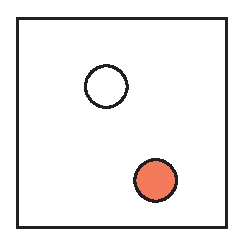
\includegraphics[width=1.5in]{sample.eps}
%  \caption{Lookit! Lookit!}
%}

%% Abstract section.
\abstract{This template aims to provide a structure and clarification on information required for submission to the IEEE VIS workshop track.
%%
Please do not alter the section order or remove sections, that are not marked as optional, but feel free to chose your own superstructure within the sections.
%%
A proposal should not exceed \textbf{four pages} and be submitted via PCS \url{https://new.precisionconference.com/vgtc}.
%%
Further information on formatting guidelines can be found at  \url{https://tc.computer.org/vgtc/publications/conference}.
%%
Please refer to the conference website for further information \url{https://ieeevis.org/year/2026/info/call-participation/workshops/}
} % end of abstract

%% Copyright space is enabled by default as required by guidelines.
%% It is disabled by the 'review' option or via the following command:
\nocopyrightspace

%%%%%%%%%%%%%%%%%%%%%%%%%%%%%%%%%%%%%%%%%%%%%%%%%%%%%%%%%%%%%%%%
%%%%%%%%%%%%%%%%%%%%%% START OF THE PAPER %%%%%%%%%%%%%%%%%%%%%%
%%%%%%%%%%%%%%%%%%%%%%%%%%%%%%%%%%%%%%%%%%%%%%%%%%%%%%%%%%%%%%%%%

\begin{document}

%% The ``\maketitle'' command must be the first command after the
%% ``\begin{document}'' command. It prepares and prints the title block.

\firstsection{Introduction, Workshop Motivation, and Goals}

\maketitle

% ----------------------------------------------------------------------
% Introduction starts here:

Besides providing a compelling title, tt the beginning of the submission, please provide an introduction to the topic covered by your workshop, including a \textbf{brief description of the workshop's motivation and goals}, e.g.,
\begin{itemize}
    \item \textbf{How will this workshop help grow} the VIS community’s intellectual horizons?
    \item \textbf{What gaps} in the main conference content or tracks will this workshop fill?
    \item \textbf{What communities} may be supported by this workshop that may not be well represented by the main conference?
\end{itemize}


% ----------------------------------------------------------------------
\section{Planned Activities and Program Outline}

Provide a concise (as concise as possible) \textbf{schedule} for a half-day or full-day event.
%%
Note that workshops are typically only half-day events, so a full-day request requires a well-reasoned justification.
%%
List \textbf{sessions, coffee breaks, and discussion periods}.
%%
Describe how these activities facilitate \textbf{active participation} by attendees, e.g., through group discussions, panels, breakouts, and/or interactive demos.
%%
If the event largely follows a traditional paper presentation format, briefly justify this choice and explain why alternative formats are less suitable.
%%
If applicable, list potential invitees for keynote/capstone presentations or panelists.

% ----------------------------------------------------------------------
\section{Evaluation of Previous Offerings (if applicable)}

If the workshop has been held previously, provide a brief evaluation of prior offerings.
%%
This evaluation should include a robust rationale for why the workshop needs to be held again and, what lessons have been learned from prior runs and how these lessons have been applied to the proposed program.

% ----------------------------------------------------------------------
\section{Definition of Success}

Define \textbf{how success will be measured} for this workshop, that is, how might the organizers evaluate whether the workshop has made progress towards addressing the original goals and motivation, e.g., number and diversity of participants, quality of discussions, and follow-up collaborations.
%%
Describe what data may be collected to assess outcomes and include a \textbf{backup policy} if success metrics targets are not met, e.g., changing the event format, or voluntarily withdrawing the event before acceptance notification is sent. 
%%
This should not require the organizers to submit emergency papers to their own event.

% ----------------------------------------------------------------------
\section{Organizer Details}
Provide \textbf{names and contact info}, including affiliations, as well as \textbf{brief bios}, relevant \textbf{related publications}, and \textbf{areas of expertise/research interests}.


% ----------------------------------------------------------------------
\section{Contributors and Diversity Plan}

Describe how you will develop and \textbf{select your list of contributors}, e.g., paper authors, speakers, panelists, etc., including \textbf{selection criteria, number, and timeline}.
%%
Explain what steps are taken to \textbf{encourage a diversity of contributors} in the workshop such as a balance of experience, background, gender, etc., with the aim of making participation as inclusive as possible.
%%
Mention efforts to attract and/or incorporate members from the practitioner community and research communities external to IEEE VIS.

% ----------------------------------------------------------------------
\section{Archival Content and Publication Plan}

State whether the workshop will have archival content (papers, reports, artworks, etc.) and plan for publication. 
%%
Refer to publication options as listed on the VGTC workshop classes page: \url{https://ieeevis.org/year/2026/info/call-participation/workshops/#workshops-with-accepted-papers}.

% ----------------------------------------------------------------------
\section{Technology and Room Requirements}

(Specify special technology needs: e.g., projectors, internet access, displays, outslets, etc. 
%%
Include in-person room configuration needs, e.g., chairs, tables, stages, etc.

% ----------------------------------------------------------------------
\section{Poster Slots}

Indicate if, and if so, estimate how many poster slots are requested.

% ----------------------------------------------------------------------
\section{Proposed Timeline}

Provide the dates for the \textbf{call for participation}, \textbf{author notification}, and \textbf{camera-ready deadlines}.
%%
Author notification must be prior to the early registration deadline for IEEE VIS.
%%
For inclusion of materials on IEEE Xplore and/or the downloadable proceedings, the camera-ready deadline must be prior to \textbf{August 19, 2026}.

% ----------------------------------------------------------------------
\section{Further Remarks (If Applicable)}

If you think that there are important aspects about this workshop submission, that cannot be suitably covered by the previous structure of the proposal, please add this information here.



% ----------------------------------------------------------------------


%\bibliographystyle{abbrv}
\bibliographystyle{abbrv-doi}
%\bibliographystyle{abbrv-doi-narrow}
%\bibliographystyle{abbrv-doi-hyperref}
%\bibliographystyle{abbrv-doi-hyperref-narrow}

\bibliography{template}
\end{document}
